\begin{figure}[ht]
 \centering
 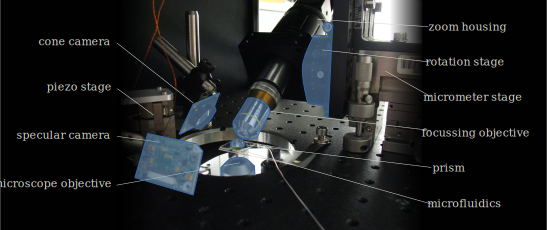
\includegraphics[keepaspectratio]{experimental/figures/spr_annotatedexperiment.pdf}
 \caption{Image of the experimental setup with the functional
  components annotated.}
\label{fig:experimentalpicture}
\end{figure}

Excitation of surface plasmon polaritions was carried out using a modified
Kretschmann attenuated total reflection (\gls{atr}) setup configuration, shown
annotated in \Figure{fig:experimentalpicture} and schematically in
\Figure{fig:experimentalsetup}.  Light from a \SI{50}{\milli\watt}
\SI{660}{\nano\meter} diode laser (Ingis 660, Laser Quantum Ltd.) with
a bandwidth of \SI{30}{\giga\hertz} is first coupled into a single mode
optical fiber via an integrated air-spaced doublet fiber collimator.  The
fiber guides the laser light to an optical breadboard mounted on an inverted
microscope.  All primary functions of the experimental setup take place on the
breadboard.  At the breadboard stage, the Gaussian beam from the single mode
fiber is collimated by an output coupler to a beam waist of
$w_0=\SI{5}{\milli\meter}$ and proceeds through a polarizing beamsplitter,
passing $p$ polarized light.  The light is focused by a 10X microscope
objective (Olympus plan achromat, $\mathrm{NA}=0.25$, \SI{10.6}{\milli\meter}
working distance) onto the hypotenuse of a hemispherical prism of diameter
$d=\SI{10}{\milli\meter}$.  The beamsplitter and microscope objective are
mounted on a rotation stage which itself is mounted on a micrometer stage.
The objective itself is mounted on a zoom housing enabling linear travel along
the optical axis, greatly simplifying the task of focussing.  When the
rotation stage is at the surface plasmon resonance angle, the micrometer $z$
axis is fixed with a near-diffraction limited spot at the center of the
prism's hypotenuse.  The spot size is modified via the zoom housing, and its
transverse location on the surface by the $x$ and $y$ lead screws on the
micrometer stage.

\begin{figure}[ht]
\centering
 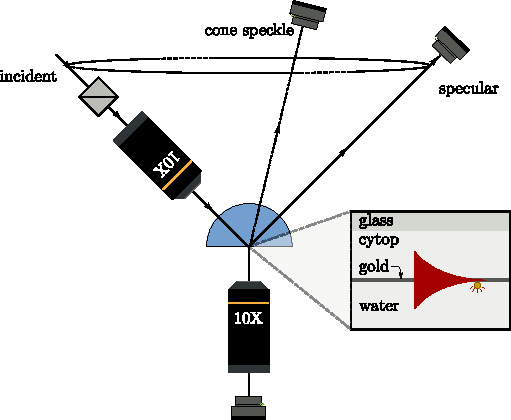
\includegraphics[keepaspectratio]{experimental/figures/conefig.pdf}
 \caption{Schematic of the experimental setup.  Description in text.}
\label{fig:experimentalsetup}
\end{figure}

The hemispherical prism is mounted on a planar structure supporting either
traditional or long-range \glspl{spp}.  A microfluidic flow cell permitting the
introduction of samples is integrated into the setup.  Both the microfluidics
and the substructure supporting the prism are thin and optically transparent.
In this way, the sensing surface may be imaged with the objective on the
inverted microscope.  The breadboard containing the experiment was fixed to
the optical table with its own micrometer stage, permitting translation of the
entire experiment in the plane of the optical table, and thus creating a way
to position the inverted microscope objective without disturbing the rest of
the setup.

The hemispherical prism affords a useful optical feature in the setup.  If the
focal spot is positioned at the central point of the hemispherical prism's
hypotenuse and the focussing optic obeys the sine condition, a minimum amount
of abberation will be introduced by the presence of the hemispherical prism.
To take advantage of this feature, a microscope objective was chosen to as the
focussing optic.  The use of a microscope objective and hemispherical prism is
not strictly necessary; previous versions of the experimental setup made use
of an $f=\SI{25}{\milli\meter}$ aspheric lens for focussing and
a \SI{25}{\milli\meter} diameter, $f=\SI{20}{\milli\meter}$ aspheric condenser
lens as an ersatz hemispherical prism.  The aspheric focussing and condenser
lens does distort the incident and reflected light precluding a diffraction
limited spot, however for the present purposes the performance difference is
not important.

Extra attention was not given to mechanical stability.  Though the quality of
the optomechanical components was acceptable, the mounting of the imaging
sensors and the prism extended on its glass slide were less than what would
typically be considered optically rigid.  Despite this, no effects were
observed on the specular or cone sensor which could be attributed to
mechanical instability, however the image from the inverted microscope
objective exhibited low frequency ($<\SI{5}{\hertz}$, measured by imaging)
displacements coincident with transient events in the laboratory: footsteps,
opening and shutting of doors, etc.  When present, such artifacts were
corrected for in a post-processing step using stabilization functions from the
software program Fiji~\cite{schindelin2012fiji}.

\subsection{Imaging Sensor}

Three identical IDS USB 2.0 \SI{8}{\bit} CMOS sensors with a spatial
resolution of $1280\times1024$ pixels operated in parallel to acquire data.
The sensors included a reduced ``area of interest'' (AOI) capture mode,
allowing a subset of the available pixel region to be transmitted via the
serial bus to the host computer.  Under this mode the cone, specular, and
surface images were captured at approximately \SI{100}{fps} and a minimum of $1280\times250$ pixels.

To allow the cone sensor to capture the largest angular region of the cone
possible, the sensor was removed from its housing and its naked PCB used as
a mount support (\Figure{fig:imagingsensor}).  Removing the housing allowed
the cone sensor to be positioned approximately \SI{10}{\milli\meter} from
the focal spot and to capture an angular region of approximately
\SI{37}{\degree}.
\begin{figure}[ht]
 \centering
 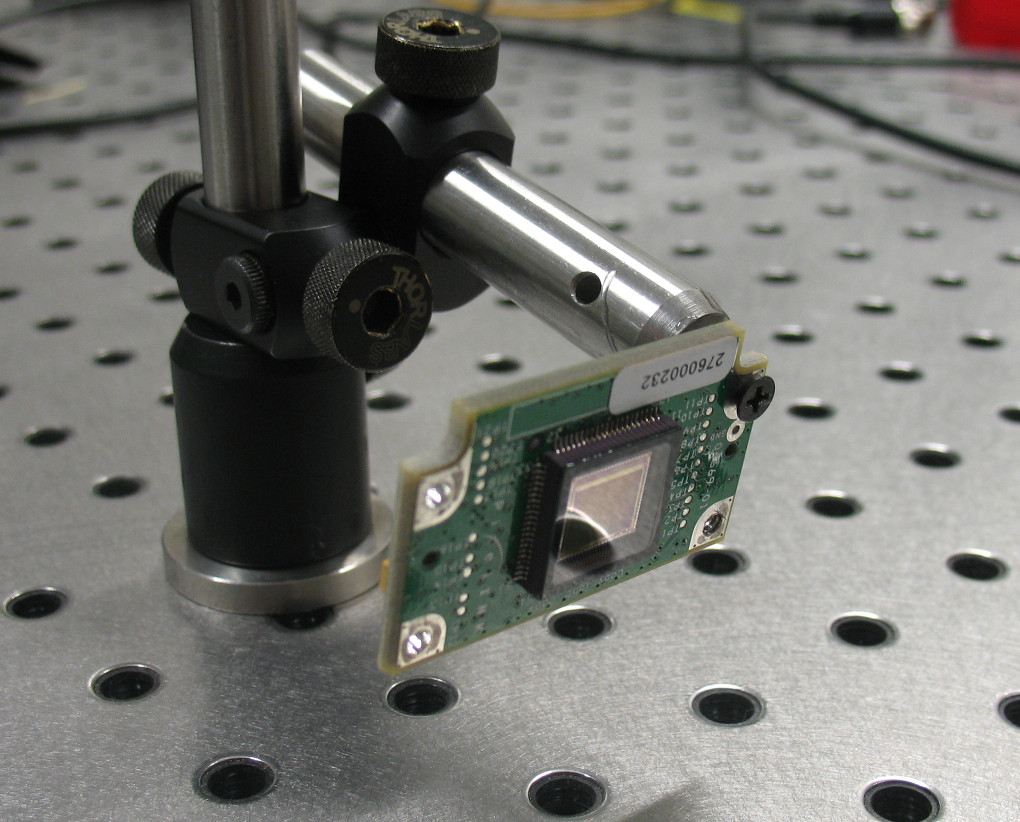
\includegraphics[width=9cm,keepaspectratio]{experimental/figures/nakedsensorcrop.jpg}
\caption{The cone sensor, an IDS USB 2.0 \SI{8}{\bit} CMOS sensor, removed from its housing allowing close positioning with respect to the prism.}
\label{fig:imagingsensor}
\end{figure}

A custom software, written in \texttt{c} and utilizing the IDS UEye SDK
version 3.82, was used to read the raw sensor data directly from memory and
write it to a single binary file on the disk of the host computer.  The
modifications increased the data acquisition speed significantly compared with
the stock software included with the IDS sensors.  This was accomplished by
first suppressing all calls image or video library calls by removing the need
to transcode the pixel data, instead writing raw pixel data directly to disk.
Second, the raw pixel data was saved to a single file, eliminating seeking of
the computer's physical disk read/write head during both file creation and
updating the disk's filesystem journal when acquiring data as an image
sequence.

On the hardware side, each imaging sensor was given its own dedicated USB
bus, maximizing the USB polling frequency and avoiding other bus traffic
which would otherwise retard the sensor datastream.

